\documentclass[11pt]{article}
\usepackage{xltxtra}
\usepackage{bookmark}
\usepackage{hyperref}
\hypersetup{hidelinks}
\usepackage{url}
\urlstyle{tt}
\usepackage{multicol}
\usepackage{xcolor}
\usepackage{calc}
\usepackage{graphicx}
\usepackage{tikz}
\usetikzlibrary{calc}
\usepackage{fontspec}
\usepackage{xeCJK}
\usepackage{relsize}
\usepackage{xspace}
\usepackage{fontawesome5}
\usepackage{titlesec}
\usepackage{enumitem}
\usepackage{siunitx}
\usepackage{amssymb}
\usepackage{tabularx}
\usepackage{multicol}
\usepackage{fontspec}
\usepackage{fancybox}
\usepackage{float}

% 取消中文字符与数字之间的间隔
\CJKsetecglue{}
\protected\def\Cpp{{C\nolinebreak[4]\hspace{-.05em}\raisebox{.28ex}{\relsize{-1}++}}\xspace}
\setlength{\parindent}{0pt}
\pagenumbering{gobble}
\setlist[itemize]{topsep=0em, leftmargin=*}
\setlist[enumerate]{topsep=0em, leftmargin=*}

% ========== 标题格式设置（改为黑体） ==========
% 一级标题：黑体，大号，加粗
\titleformat{\section}
{\LARGE\bfseries\sffamily\raggedright}  % \sffamily 使用无衬线字体（黑体）
{}{0em}
{}
[{\color{WHU_Blue}\titlerule}]
\titlespacing*{\section}{0cm}{*1}{*1}

% 二级标题：黑体，较大，加粗
\titleformat{\subsection}
{\large\bfseries\sffamily\raggedright}  % \sffamily 使用无衬线字体（黑体）
{}{0em}
{}
[]
\titlespacing*{\subsection}{0cm}{*1}{*1}

\usepackage[
a4paper,
left=1.2cm,
right=1.2cm,
top=1.5cm,
bottom=1cm,
nohead
]{geometry}

\renewcommand{\arraystretch}{1.2}
\linespread{1.2}
\renewcommand{\CJKglue}{\hskip 0.05em}

% ========== 字体设置 ==========
% 英文字体：Times New Roman（正文）
% 中文字体：宋体（正文）
% 标题字体：黑体（通过 \sffamily 实现）

% 设置英文字体（明确指定粗体）
\setmainfont{Times New Roman}[
BoldFont = Times New Roman Bold,
ItalicFont = Times New Roman Italic,
BoldItalicFont = Times New Roman Bold Italic,
]

% 设置无衬线字体（用于标题）
\setsansfont{Arial}[
BoldFont = Arial Bold,
]

% 设置等宽字体
\setmonofont{Courier New}[
BoldFont = Courier New Bold,
]

% 设置中文字体（明确指定粗体）
\setCJKmainfont{SimSun}[
BoldFont = SimHei,        % 宋体的粗体用黑体代替
ItalicFont = SimSun,      % 宋体通常没有斜体
]

% 设置中文无衬线字体（用于标题）
\setCJKsansfont{SimHei}[
BoldFont = SimHei,         % 黑体本身就有粗体效果
]

% 设置中文等宽字体
\setCJKmonofont{FangSong}[
BoldFont = SimHei,         % 仿宋的粗体用黑体代替
]

% 自定义主题色
\definecolor{WHU_Blue}{RGB}{0, 37, 84}

% 减小 itemize 间距
\setlist[itemize]{topsep=0pt, partopsep=0pt, parsep=0pt, itemsep=2pt, leftmargin=*}

% 填写个人信息
% 学院
\newcommand{\school}{Leyu College} 

% 联系方式
\newcommand{\contact}{
	\scriptsize
	\textcolor{white}{
		\faEnvelope \quad \href{mailto:202411079123@mail.bnu.edu.com}{202411079123@mail.bnu.edu.cn}
		\hspace{4em}
		\faPhone \quad  134-3088-6102
	}
}

%%%%%%%%%%%%%%%%%%%%
% 简历正文
%%%%%%%%%%%%%%%%%%%%
\begin{document}
	% 页眉：校标组合+学院名
	\begin{tikzpicture}[remember picture, overlay]
		\node[anchor=north, inner sep=0pt](header) at (current page.north){
			
\includegraphics[width=\paperwidth]{images/header.png}
		};
		% 左边校徽
		\node[anchor=west](school_logo) at (header.west){
			\hspace{0.5cm}
			
\includegraphics[width=0.2\textwidth]{images/北京师范大学校徽校名白色.png}
		};
		% 右边乐育书院图标
		\node[anchor=east](school_name) at(header.east){
			\hspace{0.5cm}
			
\includegraphics[width=0.15\textwidth]{images/乐育书院.png}
			\hspace{0.5cm}
		};
	\end{tikzpicture}
	\vspace{-3.5em}
	
	% 页脚，联系方式
	\begin{tikzpicture}[remember picture, overlay]
		\node[anchor=south, inner sep=0pt](footer) at (current page.south){
			
\includegraphics[width=\paperwidth]{images/footer.png}
		};
		% 联系方式
		\node[anchor=center] at(footer.center){\contact};
	\end{tikzpicture}
	
	% 背景
	\begin{tikzpicture}[remember picture, overlay]
		\node[opacity=0.05] at(current page.center){
			
\includegraphics[width=0.7\paperwidth, keepaspectratio]{images/bnu_logo_big.png}
		};
	\end{tikzpicture}
	
	% 个人信息
	\begin{figure}[h]
		% 左半边，信息
		%\begin{minipage}{1\textwidth}
			%\vspace*{-15pt}
			\section{\makebox[\widthof{\faAddressCard}][c]{\color{WHU_Blue}{\faAddressCard}}\quad Personal Information}
			\begin{tabular}{llll}
				Name: & Jikai Shi & \hspace*{40pt} %Date of Birth: & April 2006 
				Career Objective:& Mathematics Teacher\\
				Email: & 202411079123@mail.bnu.edu.cn &\hspace*{40pt} Phone:& 134-3088-6102 \\
			\end{tabular}
			
			\hspace*{6pt}Address: \hspace*{0pt} No.18, Jinfeng Road, Tangjiawan, Zhuhai City, Guangdong Province, P.R.China
			
		%\end{minipage}
		%\hspace{2em}
		% 右半边，照片
		%\vspace*{-10pt}
		%\begin{minipage}{0.12\textwidth}
		%	\setlength{\fboxsep}{0pt}
		%	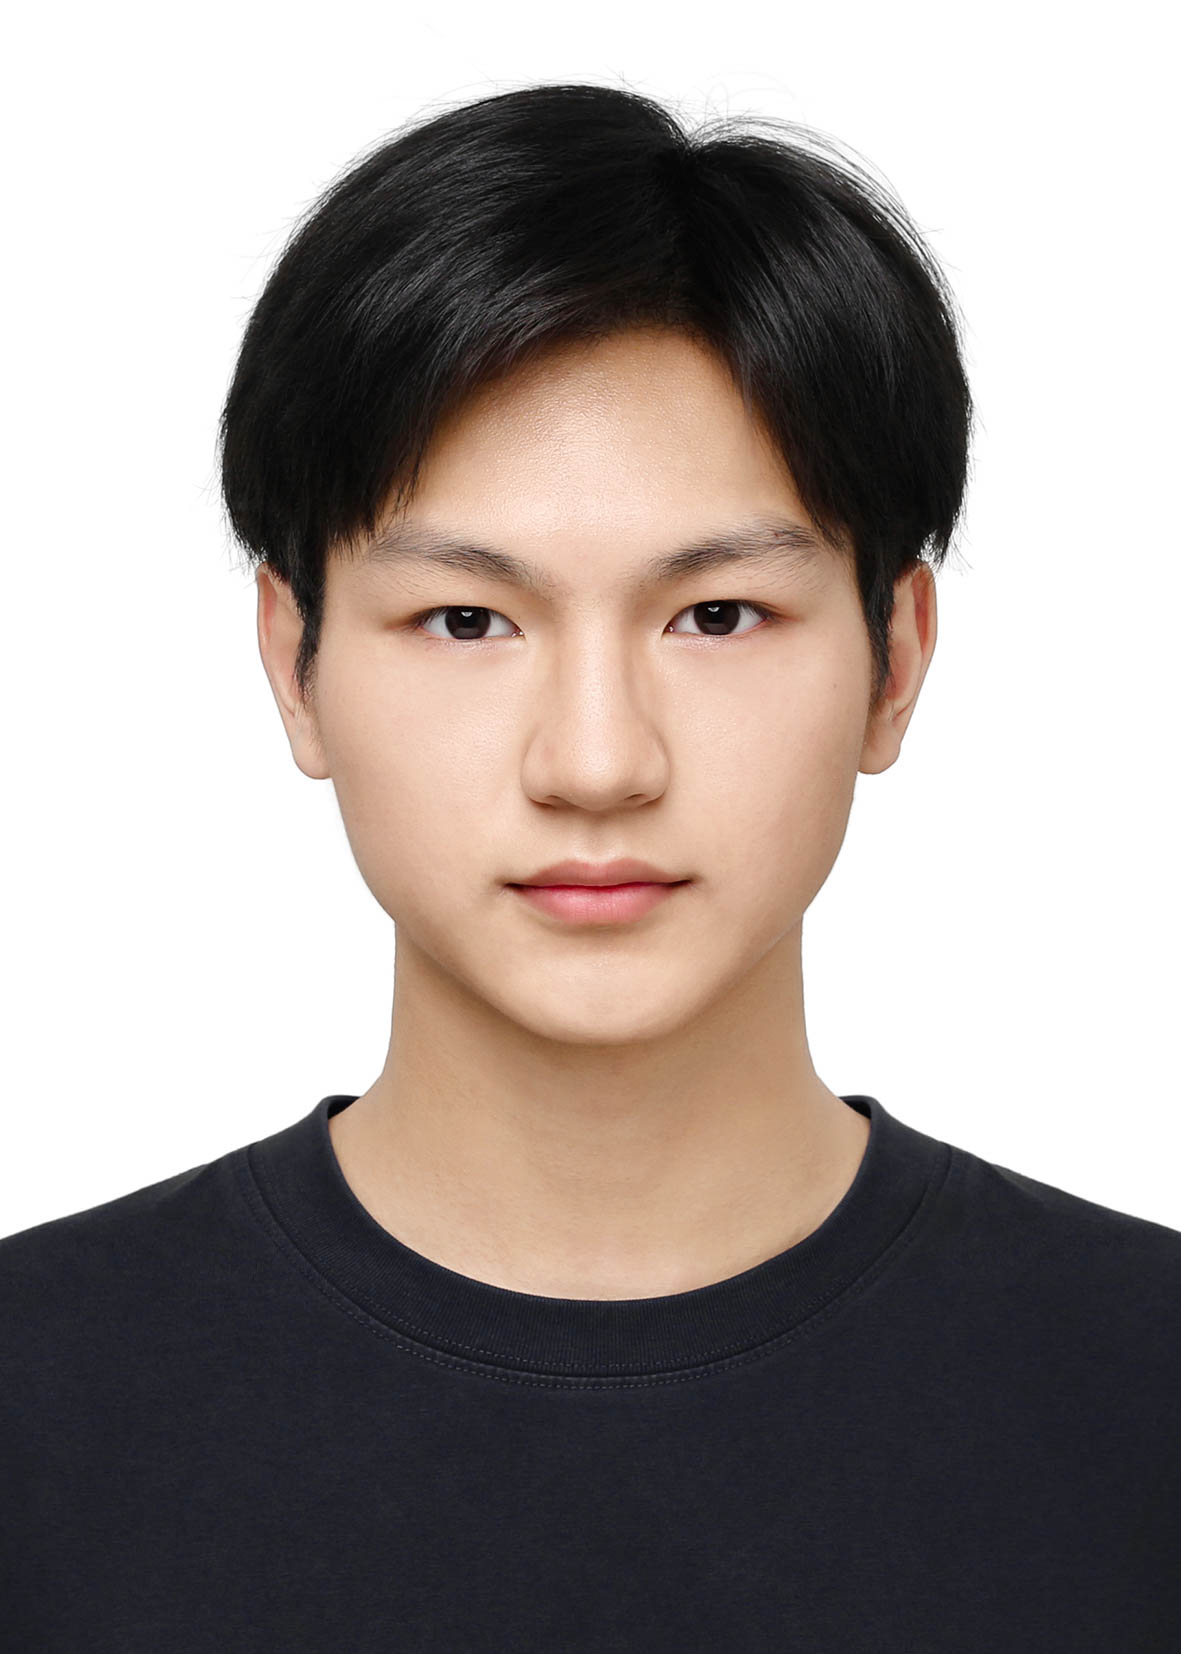
\includegraphics[width=\linewidth]{images/身份证照片Lr.png}
		%\end{minipage}
	\end{figure}
	\vspace{-1em}
	\vspace*{-5pt}
	% 教育背景
	\section{\makebox[\widthof{\faGraduationCap}][c]{\color{WHU_Blue}{\faGraduationCap}}\quad Education Background}
	
	% 教育背景（本科生）
	%{\large \textbf{Beijing Normal University}} \hspace{1.4cm} \textbf{Master} \hspace{1.6cm} \textbf{Subject Teaching (Mathematics)} \hfill {September 2028 - July 2030} 
	
	%\begin{itemize}
	
	% \item \href{学院官网.whu.edu.cn}{\underline{Ziqiang School}}，Major: Your Major  
	%	\item \textbf{Main Courses}：Mathematical Curriculum and Textbook Analysis, Mathematics Teaching Design and Case Analysis, Mathematics Education Measurement and Evaluation, Middle School Mathematics Problem Solving Research\ etc.
	%\end{itemize}
	%\vspace{0.5em}
	{\large \textbf{Beijing Normal University}} \hspace{1.2cm} \textbf{Undergraduate} \hspace{1.2cm} \textbf{Mathematics 
	%and Applied Mathematics
	} 
	\hfill September 2024 - July 2028
	
	\centering
	\textbf{(Government-sponsored Normal University Students)}
	
	\begin{itemize}
		
		\item \textbf{Main Courses}: Mathematical Analysis (83),
		 Ordinary Differential Equations (91), Pedagogy (89), %Modern Educational Technology (94), 
		 Python (96), etc.
		\item \textbf{Positions Held}: \textbf{Staff Member of the Organization Department of Leyu College Youth League Committee} (organized student group registration materials, reviewed practice reimbursement documents, served as event staff for entrance exams and award ceremonies), Vice President of Table Tennis Club, \textbf{Commissary in Charge of Publicity} (published over ten articles), Staff Member of the Text Editing Department of the Media Center
		\item \textbf{Honors and Awards}: \textbf{Third-Class Jingshi Scholarship}, \textbf{Second-Class Scholarship for Academic Achievement}
		%\item \textbf{English Proficiency}: CET-6 Score 507
		%	\item \textbf{GPA}：3.4 / 4.0（Rank 30 / 70）
	\end{itemize}
	
	\vspace{0.5em}
	%{\large \textbf{Shenzhen Second Senior High School}}\hfill September 2021 - July 2024
	
	%\begin{itemize}
	%	\item Ranked first in class, Received multiple Excellence Awards, \textbf{Top 20\% in total grade}
	%\end{itemize}
	
	%\vspace{-10pt}
	% 实践经历
	\section{\makebox[\widthof{\faGraduationCap}][c]{\color{WHU_Blue}{\faUniversity}}\quad Practical Experience}
	%	\textbf{Education Internship}
	\begin{itemize}
		\item \textbf{Volunteer Teaching "Cloud Companionship" for Tibet Support} \hfill March 2025 - August 2025 \\
		Addressed the lack of educational resources in Tibet by teaching fifth-grade mathematics online. Taught \textbf{20 lessons}, documented "Cloud Bridge Volunteer Records" and "Student Growth Portfolio". Students' final average score \textbf{increased by approximately 15 points}, received unanimous recognition from parents.
		
		\item \textbf{No. 2 Senior High School of Yanhe Tujia Autonomous County, Guizhou Province} \hfill June 2025 - July 2025 \\
		Served as an intern mathematics teacher and homeroom teacher, \textbf{taught 5 lessons}, independently completed 5 lesson plans, organized 2 unit tests, graded 60+ exam papers. Supervisor's evaluation: “\textbf{Well-structured lesson plans, clear classroom organization, strong sense of teaching responsibility.}”
	\end{itemize}
	
	
	%\vspace{-10pt}
	% 获奖情况
	\section{\makebox[\widthof{\faGraduationCap}][c]{\color{WHU_Blue}{\faTrophy}}\quad Awards and Honors}
	
	\textbf{Second Prize in “Green Bamboo” Class Teacher Skills Competition} \hfill December 2025%7
	\begin{itemize}
		\item Participated in designing \textbf{Class Management and Education Strategies} and \textbf{Theme Class Meeting Design}
		\item Represented the team in a “3-minute scenario simulation”, accurately and quickly identified the root causes of \textbf{parent-school communication problems}, efficiently completed on-site responses
	\end{itemize}
	
	
	
	
	\textbf{Provincial Third Prize in National College Mathematics Competition (Mathematics Category A)} \hfill November 2025%9
	\begin{itemize}
		\item Focused on core topics including analytic geometry, linear algebra, and mathematical analysis
		\item Mastered key modules such as vector operations, linear operators, and integral inequality proofs
	\end{itemize}
	
	
	
	
	\textbf{Provincial Third Prize in National College Mathematical Contest in Modeling} \hfill September 2025
	\begin{itemize}
		\item Responsible for modeling, programming, and paper writing
		\item Analyzed \textbf{NIPT (Non-invasive Prenatal Testing)} data for core issues related to maternal and fetal testing
		\item Constructed \textbf{Linear Mixed Models}, \textbf{Improved Canopy-Kmeans}, and \textbf{CART Decision Trees} to analyze fetal Y chromosome concentration, determine optimal testing time points, and identify abnormal female fetuses. Authored paper \textit{“Analysis of NIPT Timing Selection and Maternal/Fetal Risk”}, awarded Provincial Third Prize.
	\end{itemize}
	
	
	
	%\textbf{Third Normal University Student Culture Festival \textbf{Second Prize in Blackboard Writing Design}, \textbf{Third Prize in Lesson Plan Design}, \textbf{Third Prize in Beautiful Three-Character Writing Competition}}\hfill March 2025
	%\begin{itemize}
	%	\item Won second prize for blackboard design and third prize for corresponding review lesson plan on "Space Vectors and Solid Geometry"
	%	\item Won third prize in the chalk writing category for the poem "Untitled"
	%\end{itemize}
	
	
	% 工作技能
	%\vspace*{-10pt}
	\section{\makebox[\widthof{\faGraduationCap}][c]{\color{WHU_Blue}{\faWrench}}\quad Professional Skills}
	\begin{itemize}
		%	\item Teacher Qualification Certificate: High School Mathematics, Passed
		\item Putonghua Proficiency Level 2-A, CET-6 Score 507
		\item Proficient in Microsoft Office, as well as professional software such as LaTeX, MATLAB, Maple, VScode
		%	\item Programming: Matlab，Python，c
	\end{itemize}
	
\end{document}